% Copyright 2015 Jonathan Eyolfson
%
% This work is licensed under a Creative Commons Attribution-ShareAlike 4.0
% International License. You should have received a copy of the license along
% with this work. If not, see <http://creativecommons.org/licenses/by-sa/4.0/>.

\documentclass[10pt]{book}

\usepackage{amsmath}
\usepackage{fontspec}
\usepackage[a5paper, margin=2cm]{geometry}
\usepackage[newfloat]{minted}
\usepackage{tikz}

\setmainfont[Ligatures=TeX]{Tinos}
\setsansfont{Arimo}[Scale=MatchLowercase]
\setmonofont{Cousine}[Scale=MatchLowercase]

\definecolor{solarizedBase03}{RGB}{0, 43, 54}
\definecolor{solarizedBase0}{RGB}{131, 148, 150}
\definecolor{solarizedBlue}{RGB}{38, 139, 210}

\usetikzlibrary{decorations.pathreplacing}

\begin{document}

  \begin{titlepage}
    \begin{tikzpicture}[remember picture, overlay]
      \draw[draw=none, fill=solarizedBase03]
        (current page.north west) rectangle (current page.south east);
      \node[color=solarizedBlue, text width=1.75cm, text centered, scale=8]
        (title) at (current page.center) {\texttt{The Big Book of Computing}};
      \node[anchor=south west, inner sep=4mm, color=solarizedBase0, scale=2]
        at (current page.south west) {\textsf{0.0.1-development}};
      \node[anchor=south east, inner sep=4mm, color=solarizedBase0, scale=2]
        at (current page.south east) {\textsf{Jonathan Eyolfson}};
    \end{tikzpicture}
  \end{titlepage}

  \tableofcontents

  \chapter{Mathematical Basics}

Understand the following terminology: commutativity, and associativity.

\section{Numeral Systems}

\subsection{Decimal}

The number system you're use to is base 10. A number such as 101 can be broken
down by looking at the value associated with every digit. The numeral system
we're all familiar with is base 10. We start by associating the last digit with
the value 1 ($10^0$) and increase this value by a factor of 10 for each digit
as we work from right to left. We can break down 101 in the following chart:

\begin{center}
  \begin{tabular}{r | r | r}
    $10^2$ & $10^1$ & $10^0$ \\
    \hline
         1 &      0 &      1 \\
  \end{tabular}
\end{center}

\label{sec:numeral-system-binary}
\subsection{Binary}

\begin{center}
  \begin{tabular}{r | r | r}
    $2^2$ & $2^1$ & $2^0$ \\
    \hline
        1 &      0 &      1 \\
  \end{tabular}

  \vspace{1em}

  $= 2^2 \times 1 + 2^1 \times 0 + 2^0 \times 1 = 4 \times 1 + 1 \times 1 = 5
   = (101)_2$
\end{center}

\subsection{Octal}

This is the same as before, except now it's base 8.

\subsection{Hexadecimal}

Same as binary and octal, except instead of base 2 you use base 16.

\begin{tabular}{c c}
  \hline
  Value & Equivalent \\
  \hline
  10 & $(\text{A})_{16}$ \\
  11 & $(\text{B})_{16}$ \\
  12 & $(\text{C})_{16}$ \\
  13 & $(\text{D})_{16}$ \\
  14 & $(\text{E})_{16}$ \\
  15 & $(\text{F})_{16}$ \\
\end{tabular}

For instance: $95 = (5\text{F})_{16}$.

  \chapter{Booleans}

\section{Algebra}

\subsection{Basics}

There are 3 basic operations: \textbf{and}, \textbf{or}, and \textbf{not}. These
3 operations may go by their fancier names: \textbf{conjunction},
\textbf{disjunction}, and \textbf{negation}. The mathematical shorthand for
these 3 operations are: $\land$, $\lor$, and $\lnot$.

The first 2 operations take two booleans and produce another boolean value
(similar to addition for numbers). Since the value of a boolean can only be 0 or
1, we can enumerate all the different possibilities for these operations.  This
is shown in a truth table below:

\begin{center}
  \begin{tabular}{r r | r | r}
    $x$ & $y$ & $\land$ & $\lor$ \\
    \hline
    0 &   0 &       0 &      0 \\
    0 &   1 &       0 &      1 \\
    1 &   0 &       0 &      1 \\
    1 &   1 &       1 &      1 \\
  \end{tabular}
\end{center}

The last operation, \textbf{not}, takes one boolean value and changes its
value. So, $\lnot 0 = 1$ and $\lnot 1 = 0$.

\subsection{Derived}

There are 3 dervied operations: \textbf{equivalence}, \textbf{exclusive or
(xor)}, and \textbf{material implication}. The mathematical shorthand for these
3 operations are: $\equiv$, $\oplus$, and $\to$. Their truth table is shown
below:

\begin{center}
  \begin{tabular}{r r | r | r | r}
    $x$ & $y$ & $\equiv$ & $\oplus$ & $\to$ \\
    \hline
    0 &   0 &        1 &        0 &     1 \\
    0 &   1 &        0 &        1 &     0 \\
    1 &   0 &        0 &        1 &     1 \\
    1 &   1 &        1 &        0 &     1 \\
  \end{tabular}
\end{center}

  \chapter{Encodings}

First rule: everything in computing is a number. Everything boils down to a
sequence of booleans. When talking about booleans stored on a computer we use
the synonym bit instead. A bit is short for binary digit, which is either 0 or
1. The smallest unit stored on a computer is typically 8 bits (8 b), this unit
is called a byte (1 B).

\section{Numbers}

Unlike in pure mathematics where we can write numbers up to infinity we are
constrained by bytes on a computer. Doing strict math can easily result in
errors and wrong results. We need to be able to understand these issues so we do
not produce incorrect answers.

\begin{quote}
  “An ounce of prevention is worth a pound of cure.”

  --- Benjamin Franklin
\end{quote}

\subsection{Naturals}

The values here are exactly like the binary numeral system in
\textbf{Section~\ref{sec:numeral-system-binary}}.

\subsection{Integers}

The most popular integer encoding is \textbf{two's complement}. The sign is
encoded in the \textbf{most significant bit (MSB)}. A value of 0 indicates the
number is positive and the value is the same as the natural number value of the
remaining bits. A value of 1 indicates the number is negative and the value is
obtained from negating all the bits, adding one, and taking the value as the
natural number value of all the bits.

\newpage
\section{Character}

\subsection{ASCII}

{\scriptsize\ttfamily\begin{tabular}{c c}
  \hline
  Value & Meaning \\
  \hline
    0 & \colorbox{gray}{NUL} \\
    1 & \colorbox{gray}{SOH} \\
    2 & \colorbox{gray}{STX} \\
    3 & \colorbox{gray}{ETX} \\
    4 & \colorbox{gray}{EOT} \\
    5 & \colorbox{gray}{ENQ} \\
    6 & \colorbox{gray}{ACK} \\
    7 & \colorbox{gray}{BEL} \\
    8 & \colorbox{gray}{BS} \\
    9 & \colorbox{gray}{HT} \\
   10 & \colorbox{gray}{LF} \\
   11 & \colorbox{gray}{VT} \\
   12 & \colorbox{gray}{FF} \\
   13 & \colorbox{gray}{CR} \\
   14 & \colorbox{gray}{SO} \\
   15 & \colorbox{gray}{SI} \\
   16 & \colorbox{gray}{DLE} \\
   17 & \colorbox{gray}{DC1} \\
   18 & \colorbox{gray}{DC2} \\
   19 & \colorbox{gray}{DC3} \\
   20 & \colorbox{gray}{DC4} \\
   21 & \colorbox{gray}{NAK} \\
   22 & \colorbox{gray}{SYN} \\
   23 & \colorbox{gray}{ETB} \\
   24 & \colorbox{gray}{CAN} \\
   25 & \colorbox{gray}{EM} \\
   26 & \colorbox{gray}{SUB} \\
   27 & \colorbox{gray}{ESC} \\
   28 & \colorbox{gray}{FS} \\
   29 & \colorbox{gray}{GS} \\
   30 & \colorbox{gray}{RS} \\
   31 & \colorbox{gray}{US} \\
\end{tabular}
\quad
\begin{tabular}{c c}
  \hline
  Value & Meaning \\
  \hline
   32 & \colorbox{gray}{SPACE} \\
   33 & ! \\
   34 & " \\
   35 & \# \\
   36 & \$ \\
   37 & \% \\
   38 & \& \\
   39 & ' \\
   40 & ( \\
   41 & ) \\
   42 & * \\
   43 & + \\
   44 & , \\
   45 & - \\
   46 & . \\
   47 & / \\
   48 & 0 \\
   49 & 1 \\
   50 & 2 \\
   51 & 3 \\
   52 & 4 \\
   53 & 5 \\
   54 & 6 \\
   55 & 7 \\
   56 & 8 \\
   57 & 9 \\
   58 & : \\
   59 & ; \\
   60 & < \\
   61 & = \\
   62 & > \\
   63 & ? \\
\end{tabular}
\quad
\begin{tabular}{c c}
  \hline
  Value & Meaning \\
  \hline
   64 & @ \\
   65 & A \\
   66 & B \\
   67 & C \\
   68 & D \\
   69 & E \\
   70 & F \\
   71 & G \\
   72 & H \\
   73 & I \\
   74 & J \\
   75 & K \\
   76 & L \\
   77 & M \\
   78 & N \\
   79 & O \\
   80 & P \\
   81 & Q \\
   82 & R \\
   83 & S \\
   84 & T \\
   85 & U \\
   86 & V \\
   87 & W \\
   88 & X \\
   89 & Y \\
   90 & Z \\
   91 & [ \\
   92 & \textbackslash \\
   93 & ] \\
   94 & \textasciicircum \\
   95 & \_ \\
\end{tabular}
\quad
\begin{tabular}{c c}
  \hline
  Value & Meaning \\
  \hline
   96 & ` \\
   97 & a \\
   98 & b \\
   99 & c \\
  100 & d \\
  101 & e \\
  102 & f \\
  103 & g \\
  104 & h \\
  105 & i \\
  106 & j \\
  107 & k \\
  108 & l \\
  109 & m \\
  110 & n \\
  111 & o \\
  112 & p \\
  113 & q \\
  114 & r \\
  115 & s \\
  116 & t \\
  117 & u \\
  118 & v \\
  119 & w \\
  120 & x \\
  121 & y \\
  122 & z \\
  123 & \{ \\
  124 & | \\
  125 & \} \\
  126 & \textasciitilde \\
  127 & \colorbox{gray}{DEL} \\
\end{tabular}}

\newpage
\section{Data}

\subsection{Base64}

The following is a table of the encoded values:

{\ttfamily\begin{tabular}{c c}
  \hline
  Value & ASCII Character \\
  \hline
   0 & A \\
   1 & B \\
   2 & C \\
   3 & D \\
   4 & E \\
   5 & F \\
   6 & G \\
   7 & H \\
   8 & I \\
   9 & J \\
  10 & K \\
  11 & L \\
  12 & M \\
  13 & N \\
  14 & O \\
  15 & P \\
  16 & Q \\
  17 & R \\
  18 & S \\
  19 & T \\
  20 & U \\
  21 & V \\
  22 & W \\
  23 & X \\
  24 & Y \\
  25 & Z \\
  26 & a \\
  27 & b \\
  28 & c \\
  29 & d \\
  30 & e \\
  31 & f \\
\end{tabular}
\quad
\begin{tabular}{c c}
  \hline
  Value & ASCII Character \\
  \hline
  32 & g \\
  33 & h \\
  34 & i \\
  35 & j \\
  36 & k \\
  37 & l \\
  38 & m \\
  39 & n \\
  40 & o \\
  41 & p \\
  42 & q \\
  43 & r \\
  44 & s \\
  45 & t \\
  46 & u \\
  47 & v \\
  48 & w \\
  49 & x \\
  50 & y \\
  51 & z \\
  52 & 0 \\
  53 & 1 \\
  54 & 2 \\
  55 & 3 \\
  56 & 4 \\
  57 & 5 \\
  58 & 6 \\
  59 & 7 \\
  60 & 8 \\
  61 & 9 \\
  62 & + \\
  63 & / \\
\end{tabular}}

Each encoded value represents 6 bits. Each group is 4 characters long.
Therefore these 4 characters represent 3 bytes (`=' is used for padding).

  \chapter{File Formats}

\section{Executable and Linkable Format (ELF)}

The ELF format is the file format for executable programs on most *NIX systems.

Comes in two formats: 32-bit and 64-bit.

\begin{center}
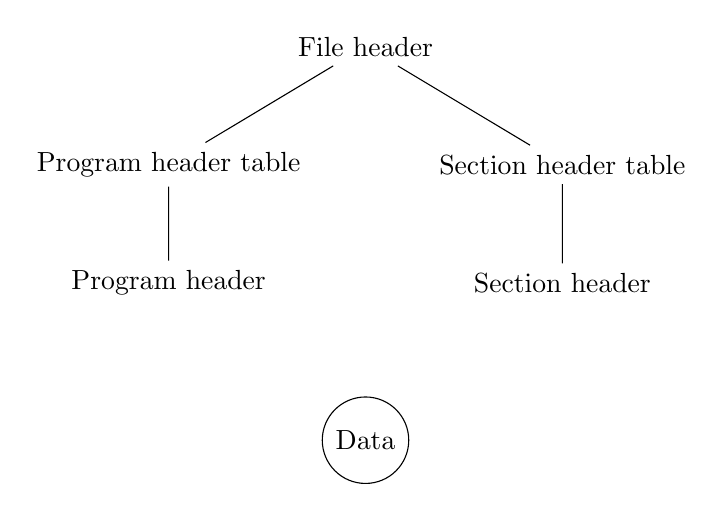
\begin{tikzpicture}[sibling distance=5cm, every node/.style={align=center}]
  \node {File header}
    child { node {Program header table}
      child { node {Program header} }
    }
    child { node {Section header table}
      child { node {Section header} }
    };

  \node [circle, draw] at (0, -5) {Data};
\end{tikzpicture}
\end{center}

\subsection{File header}

The beginning 16 bytes of the file are byte order agnostic.
The first byte must have the value $(7\text{F})_{16}$ (127) followed by
$(45)_{16}$, $(4\text{C})_{16}$, and $(46)_{16}$ (ELF in ASCII encoding).

\subsection{Program header table}

\subsection{Section header table}

This section is only used for linking(?).

  \chapter{Instruction Set Architecture}

Processors understand bytes in groups of different sizes. The representation of
this grouping is different on various processors. When we're using this data, we
understand it fully as a group and don't break it up into different parts. We
consider these groups to be \textbf{words} (their term not mine). We would
naturally understand a group of bytes with the most significant byte written to
the left writing the next least significant byte to the right. For instance, a 4
byte word is shown below with the least significant byte being 0-indexed.

\begin{center}
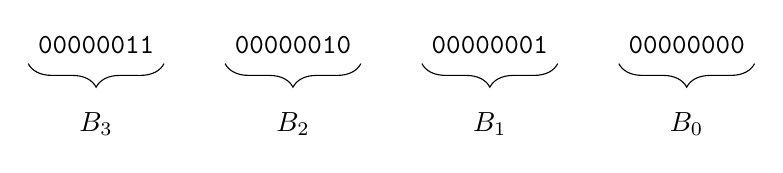
\begin{tikzpicture}
  \node (b3) {\ttfamily 00000011};
  \draw[decorate,decoration={amplitude=3mm,brace,mirror}]
    (b3.south west) -- (b3.south east);
  \node[below of=b3,anchor=center]{$B_3$};

  \node[right of=b3,node distance=2.5cm] (b2) {\ttfamily 00000010};
  \draw[decorate,decoration={amplitude=3mm,brace,mirror}]
    (b2.south west) -- (b2.south east);
  \node[below of=b2,anchor=center]{$B_2$};

  \node[right of=b2,node distance=2.5cm] (b1) {\ttfamily 00000001};
  \draw[decorate,decoration={amplitude=3mm,brace,mirror}]
    (b1.south west) -- (b1.south east);
  \node[below of=b1,anchor=center]{$B_1$};

  \node[right of=b1,node distance=2.5cm] (b0) {\ttfamily 00000000};
  \draw[decorate,decoration={amplitude=3mm,brace,mirror}]
    (b0.south west) -- (b0.south east);
  \node[below of=b0,anchor=center]{$B_0$};
\end{tikzpicture}
\end{center}

\section{ARM}

Currently, the plan is to initially make this secton specifically for ARMv7.

\section{x86-64}

\begin{listing}[H]
  \inputminted[frame=lines]{asm}{code/hello_world.asm}
  \caption{``Hello world'' program written in x86-64 assembly for Linux}
  \label{lst:hello-world-asm}
\end{listing}

Assuming the file is called ``\mintinline{console}{hello_world.asm}'' we need to
compile to machine code using \mintinline{console}{nasm -f elf64
  hello_world.asm}. This produces a file named
``\mintinline{console}{hello_world.o}'' which is an object file (more later). To
produce an executable file that will run on the machine use the standard linker:
\mintinline{console}{ld hello_world.o -o hello_world}. This produces an
executable named ``\mintinline{console}{hello_world}''. Running the program
using \mintinline{console}{./hello_world} produces the output
``\mintinline{console}{Hello world!}''.

x86-64 has 16 general purpose registers: \mintinline{asm}{rax},
\mintinline{asm}{rbx}, \mintinline{asm}{rcx}, \mintinline{asm}{rdx},
\mintinline{asm}{rbp}, \mintinline{asm}{rsi}, \mintinline{asm}{rdi},
\mintinline{asm}{rsp}, \mintinline{asm}{r8}, \mintinline{asm}{r9},
\mintinline{asm}{r10}, \mintinline{asm}{r11}, \mintinline{asm}{r12},
\mintinline{asm}{r13}, \mintinline{asm}{r14}, and \mintinline{asm}{r15}. The
stack pointer is \mintinline{asm}{rsp} and it is always(?) in use.

Note that the system call number goes in register \mintinline{asm}{rax}. Note
that (on x86-64) the system call number for \mintinline{asm}{write} is
\texttt{1} and for \mintinline{asm}{exit_group} is \texttt{231}. The arguments
to the system call go in registers according to the following table:

{\ttfamily\begin{tabular}{c c}
  \hline
  Index & Register \\
  \hline
  0 & \mintinline{asm}{rdi} \\
  1 & \mintinline{asm}{rsi} \\
  2 & \mintinline{asm}{rdx} \\
  3 & \mintinline{asm}{r10} \\
  4 & \mintinline{asm}{r8} \\
  5 & \mintinline{asm}{r9} \\
\end{tabular}}

In C, \mintinline{asm}{rcx} is used instead of \mintinline{asm}{r10} for the
argument at index 3. The kernel destroys registers in \mintinline{asm}{rcx} and
\mintinline{asm}{r11}. Registers \mintinline{asm}{rbp}, \mintinline{asm}{rbx},
\mintinline{asm}{r12}, \mintinline{asm}{r13}, \mintinline{asm}{r14}, and
\mintinline{asm}{r15} belong to the calling function and are untouched by the
kernel.

  \chapter{Parallelism}

\section{Limitations}

\subsection{Amdahl's Law}

Let $N$ be the number of parallel executions.

\noindent Let $S$ be the fraction of serial runtime for a serial execution.

\noindent Let $P$ be the fraction of parallel runtime for a serial execution.

\vspace{1em}

$\text{speedup} = \frac{1}{S + \frac{P}{N}}$

\subsection{Gustafson's Law}

Let $N$ be the number of parallel executions.

\noindent Let $n$ be a measure of the problem size.

\noindent Let $S(n)$ be the fraction of serial runtime for a parallel
execution.

\noindent Let $P(n)$ be the fraction of parallel runtime for a parallel
execution.

\vspace{1em}

$\text{speedup} = S(n) + N \cdot P(n)$


  \chapter{Linux Kernel}

  Include memory allocation declarations with
  \mintinline{c}{#include <linux/slab.h>}.

  \section{Userland API}

  \chapter{Cryptography}

  \section{Block Ciphers}

  \subsection{Modes of Operation}

  \subsubsection{Electronic Codebook (ECB)}

  \subsubsection{Cipher Block Chaining (CBC)}

  \subsubsection{Counter (CTR)}

  \chapter{Information Theory}

  \section{Hamming Distance}

  A measure of how many characters are different in two strings of equal length.

  Example: Consider the two ASCII encoded strings ``this is a test'' and ``wokka
  wokka!!!''. Both have the same length of 14 characters. If each character is
  represented as 8 bits we have to many 112 comparsions ($14 \times 8$).

  \texttt{t} is $116 = (74)_{16} = (01110100)_{2}$

  \texttt{w} is $119 = (77)_{16} = (01110111)_{2}$

  This hamming distance between these two characters is 2.

  \texttt{h} is $104 = (68)_{16} = (01101000)_{2}$

  \texttt{o} is $111 = (6\text{F})_{16} = (01101111)_{2}$

  This hamming distance between these two characters is 3, running total of 5.

  \texttt{i} is $105 = (69)_{16} = (01101001)_{2}$

  \texttt{k} is $107 = (6\text{B})_{16} = (01101011)_{2}$

  This hamming distance between these two characters is 1, running total of 6.

  And so on, the hamming distance of these two strings is 37.

\end{document}
